\documentclass[tikz, border=10pt]{standalone}
\usepackage{iftex}
\ifluatex
  \usepackage{fontspec}
  \usepackage{unicode-math}
  \setmainfont{Fira Sans}
  \setmonofont{Fira Mono}
  \setmathfont{Fira Math}
  \setmathfont{STIX Two Math}[range={"29F5,"2216}]
\else
  \usepackage[T1]{fontenc}
\fi

\usepackage{amsmath}
\usepackage{tikz}
\usetikzlibrary{arrows.meta}
\tikzset{every node/.style={font=\Large}}

% Theme toggle: \darkbgfalse for light background preview.
\newif\ifdarkbg
\darkbgfalse
\ifdarkbg
  \colorlet{axiscol}{white}
  \colorlet{gridcol}{white!30!black}
  \colorlet{ticklabelcol}{white}
  \colorlet{funcol}{yellow!85!white}
  \colorlet{auxcol}{white!50!black}
\else
  \colorlet{axiscol}{black}
  \colorlet{gridcol}{black!25!white}
  \colorlet{ticklabelcol}{black}
  \colorlet{funcol}{blue!70!black}
  \colorlet{auxcol}{black!40!white}
\fi

% x: -1 to 5  (6 units)   xscale=0.9  → ~5.4 cm wide
% y: -6 to  4  (10 units)  yscale=0.75 → ~7.5 cm tall
% f(-1) = -6  and  f(5) = -6  → parabola exits at symmetric corners.
% Vertex at (2, 3).  Axis of symmetry: x = 2.
\begin{document}
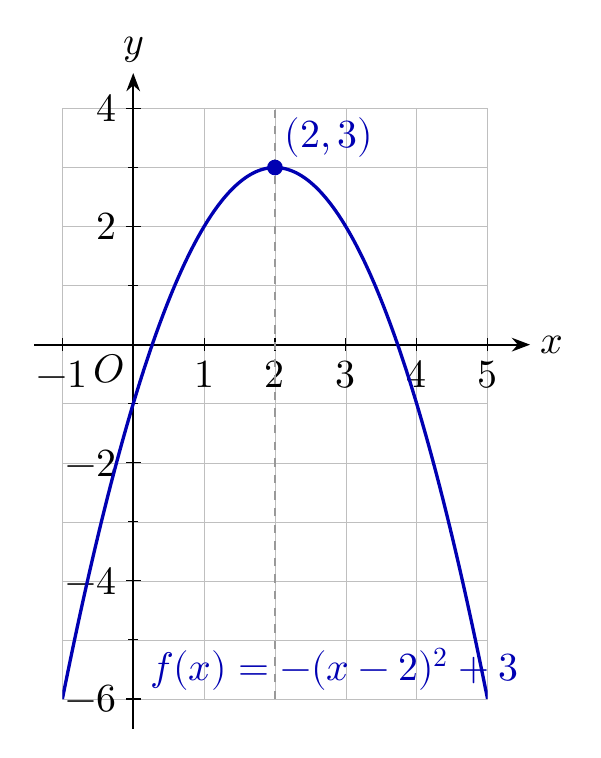
\begin{tikzpicture}[xscale=0.9, yscale=0.75, >=Stealth]

  % Cartesian grid.
  \draw[step=1, very thin, gridcol] (-1,-6) grid (5,4);

  % Axes.
  \draw[->, thick, axiscol] (-1.4,0) -- (5.6,0)
    node[right, text=axiscol] {$x$};
  \draw[->, thick, axiscol] (0,-6.5) -- (0,4.6)
    node[above, text=axiscol] {$y$};

  % Tick marks — x axis (skip 0, labeled as O).
  \foreach \x in {-1,1,2,3,4,5} {
    \draw[axiscol] (\x, 3pt) -- (\x, -3pt)
      node[below, text=ticklabelcol] {$\x$};
  }

  % Tick marks — y axis (labelled every 2, minor every 1).
  \foreach \y in {-6,-4,-2,2,4} {
    \draw[axiscol] (3pt,\y) -- (-3pt,\y)
      node[left, text=ticklabelcol] {$\y$};
  }
  \foreach \y in {-5,-3,-1,1,3} {
    \draw[axiscol] (2pt,\y) -- (-2pt,\y);
  }

  % Origin label.
  \node[below left, text=axiscol] at (0,0) {$O$};

  % Axis of symmetry x = 2 (dashed).
  \draw[dashed, auxcol] (2,-6) -- (2,4);

  % Function curve: f(x) = -(x-2)^2 + 3, clipped to the window.
  \begin{scope}
    \clip (-1,-6) rectangle (5,4);
    \draw[domain=-1:5, smooth, very thick, funcol, samples=80]
      plot (\x, {-(\x-2)^2 + 3});
  \end{scope}

  % Function label — lower-left, away from the curve.
  \node[right, text=funcol] at (0.1,-5.5) {$f(x)=-(x-2)^2+3$};

  % Vertex (2, 3) — maximum.
  \node[circle, fill=funcol, inner sep=2pt] at (2,3) {};
  \node[above right, text=funcol] at (2,3) {$(2,3)$};

  % y-intercept (0, -1).
  % \node[circle, fill=funcol, inner sep=2pt] at (0,-1) {};

  % Symmetric point (4, -1).
  % \node[circle, fill=funcol, inner sep=2pt] at (4,-1) {};

\end{tikzpicture}
\end{document}
